\documentclass{article_saj}
\pagestyle{myheadings}
\usepackage{graphicx,saj,multicol,subeqnarray}
\usepackage{natbib}
\usepackage{float}
\usepackage{xcolor}
\usepackage{widetext}
\usepackage{url}
\usepackage{bm}
\usepackage{tikz} % for checkmark
\usepackage{pifont} % for xmark
\usepackage{amsfonts}
\usepackage{amssymb}
\usepackage{amsmath,upgreek}

\usepackage{titlesec}
\def\tg{\mathop{\rm tg}\nolimits}
\def\arctg{\mathop{\rm arctg}\nolimits}

\def\point#1{\hbox{\setbox7=\hbox to0.6em{\hfil.\hfil}%
\setbox8=\hbox to0.5em{\hfil$^{#1}$\hfil}%
\box7\kern-0.5em\box8}}

\def\pointmin#1{\hbox{\setbox2=\hbox to0.8em{\hfil.\hfil}%
\setbox3=\hbox to0.6em{\hfil$^{#1}$\hfil}%
\box2\kern-.7em\box3}}

%for non integer numbers for years, days, hours, minutes and seconds

\def\yyy{\point{\mathrm{y}}}
\def\ddd{\point{\mathrm{d}}}
\def\hhh{\point{\mathrm{h}}}
\def\mmm{\pointmin{\mathrm{m}}\kern.15em}
\def\sss{\point{\mathrm{s}}}

%for non integer numbers for arc degrees, arc minutes and arc seconds

\def\oo{\point{\circ}}
\def\lll{\point{\prime}}
\def\uu{\point{\prime\prime}}

%for integer numbers for arc degrees, arc minutes and arc seconds

\def\OO{$^\circ$}
\def\LLL{$^\prime$}
\def\UU{$^{\prime\prime}$}
 

\titlelabel{\thetitle.\quad}
\definecolor{xlinkcolor}{cmyk}{1,0.6,0,0}
\usepackage[bookmarks=false,         % show bookmarks bar?
     pdfnewwindow=true,      % links in new window
     colorlinks=true,    % false: boxed links; true: colored links
     linkcolor=xlinkcolor,     % color of internal links
     citecolor=xlinkcolor,     % color of links to bibliography
     filecolor=xlinkcolor,  % color of file links
     urlcolor=xlinkcolor,      % color of external links
final=true
]{hyperref}

% Papertype can be "Invited Review", "Original Scientific Paper",
% "Preliminary report" or "Professional paper"

\def\papertype{\ \hfill\ Editorial}

\setcounter{page}{1}
\setcounter{firstpage}{1}
\setcounter{lastpage}{5}

\citestyle{kluwer}%

\setcounter{footnote}{0}
\renewcommand{\thefootnote}{\fnsymbol{footnote}}

\begin{document}
%
\parindent=.5cm
\baselineskip=3.8truemm
\columnsep=.5truecm
%

\newenvironment{lefteqnarray}{\arraycolsep=0pt\begin{eqnarray}}
{\end{eqnarray}\protect\aftergroup\ignorespaces}
\newenvironment{lefteqnarray*}{\arraycolsep=0pt\begin{eqnarray*}}
{\end{eqnarray*}\protect\aftergroup\ignorespaces}
\newenvironment{leftsubeqnarray}{\arraycolsep=0pt\begin{subeqnarray}}
{\end{subeqnarray}\protect\aftergroup\ignorespaces}
%

% Runningtitle
\markboth{\eightrm LABORATORIO DI TERMODINAMICA} 
{\eightrm LABORATORIO DI TERMODINAMICA}

\begin{strip}


%%%% INTESTAZIONE %%%%%%%%%%%%%%%%%%%%%%%%%%%%%%%%%%%%%%%%%%%%%%%%%%%%%%%%%%%%

% TITOLO
\title{
     MISURE DI CALORE SPECIFICO DI ALCUNI MATERIALI E DEL CALORE LATENTE
     DI FUSIONE DELL'ACQUA
}
% AUTORI
\authors{A. Cipriano$^{1}$, M. Cingolo$^{2}$ e P. Corrado$^{3}$}
\vskip3mm
% INFORMAZIONI AUTORI
\address{Dipartimento di Fisica, Corso di laurea in Fisica, Università di Roma 
La Sapienza\break matricole: $^1$2149050, $^2$2129732, $^3$2140217}






%%%% ABSTRACT %%%%%%%%%%%%%%%%%%%%%%%%%%%%%%%%%%%%%%%%%%%%%%%%%%%%%%%%%%%%%%%%%
\abstract{
     Il calore specifico dei materiali e il calore latente di fusione
     sono parametri fondamentali per la comprensione dei processi termodinamici. 
     In questa esercitazione di laboratorio, è stato misurato il calore specifico di diversi materiali 
     e il calore latente del ghiaccio attraverso esperimenti basati sull’equilibrio 
     termico. I materiali sono stati immersi in un thermos con acqua calda 
     fino al raggiungimento dell'equilibrio termico, e successivamente trasferiti 
     in un thermos a temperatura ambiente, misurando la temperatura inziale e finale 
     del corpo si è ricavato, tramite il primo principio della termodinamica il calore 
     specifico del materiale. Il calore latente è stato determinato sciogliendo il 
     ghiaccio in acqua a temperatura controllata. I risultati mostrano che i materiali risultano essere
     compatibili con alluminio, ottone, marmo e okite.
}
%%%%%%%%%%%%%%%%%%%%%%%%%%%%%%%%%%%%%%%%%%%%%%%%%%%%%%%%%%%%%%%%%%%%%%%%%%%%%%%



\end{strip}
\tenrm



%%%% SEZIONE 1: INTRODUZIONE %%%%%%%%%%%%%%%%%%%%%%%%%%%%%%%%%%%%%%%%%%%%%%%%%%
\section{INTRODUZIONE}
Se prendiamo in considerazione un sistema ipoteticamente isolato dall'ambiente esterno
in cui il volume rimane costante, per il primo principio della termodinamica 
\begin{equation}
     Q_1 = -Q_2
     \label{eq:1}
\end{equation}
il corpo di massa a temperatura maggiore cede calore al corpo a temperatura minore, fino al raggiungimento
della temperatura finale $T_f$ e dunque l'equilibrio termico. Se come sistema prendiamo un corpo
di massa $m_1$ a temperatura iniziale $T_1$ che viene immerso in acqua a temperatura $T_{i,acq}$
e possibile calcolare il calore specifico come:
\begin{equation}
     c_1 = \frac{c_{acq}(m_{acq} + M_e)(T_{i,acq} - T_f)}{m_1(T_f - T_1)}
     \label{eq:2}
\end{equation}
dove $c_{acq}$ è il calore specifico dell'acqua e $M_e$ la massa equivalente
del thermos, necessaria per tener conto del calore assorbito o ceduto dal thermos.
Sempre dal primo principio della dinamica è possibile ricavare il calore latente del ghiaccio:
\begin{equation}
     \lambda_g = \frac{c_{acq}[(m_{acq} + M_e)(T_{i,acq} - T_g) - m_g(T_f - T_g) ]}{m_g}
     \label{eq:3}
\end{equation}
$T_g$ è la temperatura del ghiaccio quando viene immerso nell'acqua, pari a $0^\circ C$.



\indent
%%%%%%%%%%%%%%%%%%%%%%%%%%%%%%%%%%%%%%%%%%%%%%%%%%%%%%%%%%%%%%%%%%%%%%%%%%%%%%%






%%% SEZIONE 2: APPARATO SPERIMENTALE %%%%%%%%%%%%%%%%%%%%%%%%%%%%%%%%%%%%%%%%%%
\section{APPARATO SPERIMENTALE}
\begin{itemize}
     \item \textbf{Thermos}:
          Al fine di ridurre al minimo lo scambio di 
          calore con l'ambiente esterno, e garantire che il calore venga scambiato
          solo tra i materiali coinvolti, sono stati impiegati due thermos.
     \item \textbf{Bilancia digitale}:
          Per misurare le masse dei corpi è stata impiegata una bilancia 
          digitale con sensibilità di 0.1 g.
     \item \textbf{Termometri}:
          per la misura di temperature sono stati impiegati due
          termometri a mercurio con sensibilità di 0.2 $^\circ C$
     \item \textbf{Bollitore elettrico}:
          Imiegato per portare l'acqua a temperature superiori
          a quella ambiente.
 \end{itemize}
\indent
%%%%%%%%%%%%%%%%%%%%%%%%%%%%%%%%%%%%%%%%%%%%%%%%%%%%%%%%%%%%%%%%%%%%%%%%%%%%%%%



%%% SEZIONE 3: PROCEDURA SPERIMENTALE %%%%%%%%%%%%%%%%%%%%%%%%%%%%%%%%%%%%%%%%%%
\section{PROCEDURA SPERIMENTALE}
     La procedura sperimentale è stata suddivisa in due parti, la prima 
     volta a misurare il calore specifico di alcuni materiali e la seconda 
     il calore latente dell'acqua. In entrambe gli esperimenti i valori della massa equivalnte $M_e$ 
     e del calore specifico dell'acqua sono stati $c_{acq}$ considerati noti e pari rispettivamente a $1 cal/gK$
     e $25 \pm 5$ g.
%%% CALORE SPECIFICO
\subsection{Calore specifico}
Per ogni campione di materiale analizzato é stata inizialamente misurata la massa,
in seguito il campione è stato immerso in un primo thermos contenente acqua 
ad una temperatura nel range di $ 58-67 ^\circ C$ e al raggiungimento dell'equilibrio termico è stata
misurata la temperatura dell'acqua e quindi per equazione \ref{eq:1} quella del corpo. 
Il corpo è stato in seguito trasferito in un secondo thermos, contenente acqua a temperatura iniziale $T_{i,acq}$ precedentemente
misurata. Raggiunto l'equilibrio è stata acquisita la temperatura finale $T_f$ del sistema e tramite
equazione \ref{eq:2} è stato calcolato il calore specifico.
Poichè questo procedimento viene ripetuto, la massa dell'acqua potrebbe diminuire quando
il corpo viene spostato e poi nuovamente riposto nel secondo thermos, al fine di 
tenere in considerazione le possibili variazione di massa dovute a questa procedura,
per ogni ripetizione dell'esperimento é stata misurata la massa complessiva $m_{tot} = m_{th} + m_{acq}$, del
sistema costituito dal thermos e dall'acqua, e dalla misura della massa del thermos $m_{th}$
abbiamo ottenuto, per differenza, la massa di acqua $m_{acq}$.



%%% CALORE LATENTE DI FUSIONE
\subsection{Calore latente di fusione del ghiaccio}
Inizialmente il ghiaccio si presenteva ad una temperatura di $\approx -3^\circ C$,
è stato dunque immerso in un thermos con poca acqua e tramite un termometro si è monitorata
la temperatura. Quando il termometro si è stabilizzato a $ 0 ^\circ C$, il ghiaccio é stato 
traferito nel secondo thermos, contenete acqua riscaldata tramite bollitore elettrico,
di cui è stata misurata la massa $m_{acq}$.
Misurando la temperatura iniziale $T_i$ del ghiacchio la temperatura iniziale dell'acqua $T_{i,acq}$
nel secondo termos e la temperatura $T_f$ all'equilibrio, si è ricavato tramite \ref{eq:3}
il calore latente del ghiaccio. L'esperimento è stato eseguito due volte, al fine di ottenere 
una (motivare).
\indent
%%%%%%%%%%%%%%%%%%%%%%%%%%%%%%%%%%%%%%%%%%%%%%%%%%%%%%%%%%%%%%%%%%%%%%%%%%%%%%%






%%% SEZIONE 4: RISULTATI %%%%%%%%%%%%%%%%%%%%%%%%%%%%%%%%%%%%%%%%%%%%%%%%%%%%%%
\section{RISULTATI}
Per la misura del calore specifico dell'alluminio, sono state effettuate 5 misure, mentre per gli altri materiali due.
In tabella \ref{table1} è stata riportata la media pesata con le incertezze, la deviazione standard del campione e la deviazione standard  della media.
Essendo il campione statisticamente poco rilevante a causa dell'esiguo numero di misure, è stata calcolata anche
la deviazione standard della media pesata $\sigma_p$.
Come si puo notare dal grafico in figura \ref{fig2}, 
i valori misurati, tranne il Quarzo, riusltano essere compatibili entro le incertezze sperimentali con i valori noti. Probabilmente,
oltre agli effetti sistematici, il motivo dell'incompatibilità del quarto materiale con il quarzo è dovuto al fatto che si tratta di okite, un
materiale che seppur composto principalmente da quarzo, viene miscelato con resine, vetro e materiali ferrosi che ne alterano la struttura e le propietà fisiche.
Le misure risultano essere molto grossolane, con errori assoluti anche superiori al 50 \%, questo è dovuto principalmente alla variazione di temperatura
durante l'esperimento che risulta essere molto piccola, dell'ordine di $1-2 ^\circ\text{C}$, nella misura del calore latente di fusione del ghiaccio, infatti, in cui la variazione 
di temperatura è risultata essere maggiore l'errore relativo è risultato essere molto piu basso e pari circa al 3 \%. Inoltre potrebbero essere presenti
errori sistematici dovuti alla dispersione termica di calore durante le procedure, come l'apertura e la chiusura del thermos, al fatto che il thermos non 
isola completamente il sistema dall'amabiente esterno.





\begin{figure}[ht]
     \centerline{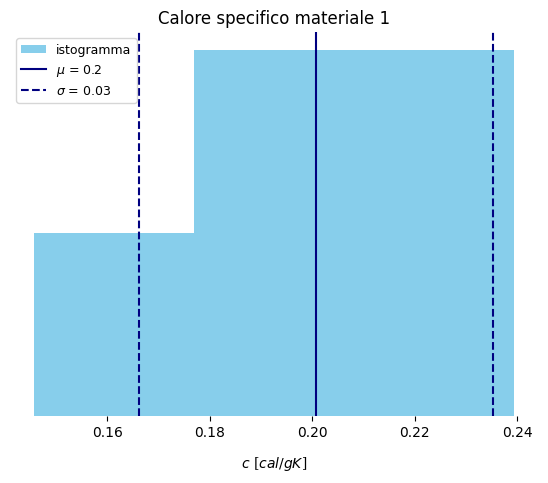
\includegraphics[width=0.9\columnwidth, keepaspectratio]{distribuzione_cs_alluminio.png}}
     \caption{Distribuzione delle 5 misure di calore specifico per il materiale 1.}
     \label{fig1}
\end{figure}

\begin{figure}[ht]
     \centerline{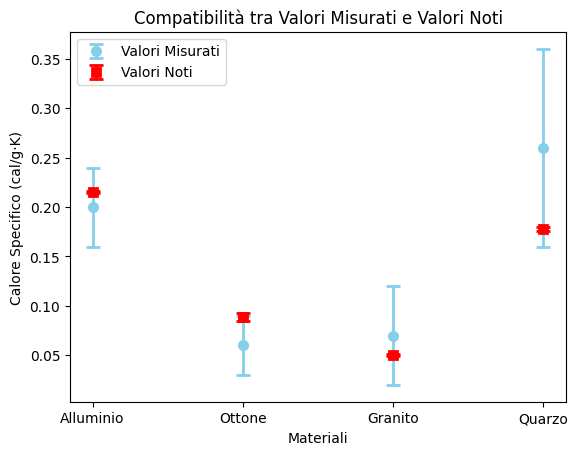
\includegraphics[width=0.9\columnwidth, keepaspectratio]{compatibilita_cs.png}}
     \caption{Compatibilità tra misure effettuate e valori noti, consultati sul sito www.matweb.com,
     in cui i valori riportati fanno riferimento al manuale CRC Handbook of Chemistry and Physics, Robert C. Weast, Ed. 62 Edition, CRC Press, Boca Raton, FL, 1981.}
     \label{fig2}
\end{figure}



\indent
%%%%%%%%%%%%%%%%%%%%%%%%%%%%%%%%%%%%%%%%%%%%%%%%%%%%%%%%%%%%%%%%%%%%%%%%%%%%%%%






%%% SEZIONE 5: CONCLUSIONI %%%%%%%%%%%%%%%%%%%%%%%%%%%%%%%%%%%%%%%%%%%%%%%%%%%%
\section{CONCLUSIONI}
Nel complesso, l'esperimento ha fornito risultati soddisfacenti per la maggior parte dei materiali testati, 
sebbene ci sia margine per migliorare la precisione e ridurre gli errori sistematici con ulteriori accorgimenti sperimentali.

\begin{table}[ht]
     \caption{{Valori del calore specifico in $cal/gK$ ottenuti per i diversi materiali analizzati.}}
     \vskip.25cm
     \centerline{\begin{tabular}{ccccc}
     \hline
     Materiale & $\mu$ & $\sigma$ & $\sigma_m$ & $\sigma_p$ \\
     \hline
     1  & 0.20 & 0.04 & 0.02 & 0.04 \\
     2  & 0.060 &  0.01 & 0.01 & 0.03 \\
     3  & 0.07 &  0.03 & 0.02 & 0.05 \\
     4  & 0.26 &  0.01 & 0.004 & 0.1 \\
 
     \hline
     \end{tabular}}
     \label{table1}
\end{table}


\begin{table}[ht]
     \caption{{Misure effettuate per il calore latente del ghiaccio. 
     le misure di masse sono riportate in g 
          mentre quelle di temperature in $^\circ\text{C}$, il calore latente del ghiaccio è invece espresso in $cal/g$}}
     \vskip.25cm
     \centerline{\begin{tabular}{cccccc}
     \hline
     $m_a $ & $T_a $ & $T_f$ & $m_g$ & $\lambda_g$ & $\sigma_{\lambda_g}$ \\
     \hline
     238.4  & 52.4 & 28.4 & 63.2 & 72 & 2\\
     231.5  & 55.0 &  24.6 & 75.6 & 78 & 3\\
 
     \hline
     \end{tabular}}
     \label{table2}
\end{table}
\indent
%%%%%%%%%%%%%%%%%%%%%%%%%%%%%%%%%%%%%%%%%%%%%%%%%%%%%%%%%%%%%%%%%%%%%%%%%%%%%%%











% References
%\vskip2mm

\newcommand\eprint{in press }

\bibsep=0pt

\bibliographystyle{aa_url_saj}

{\small

\bibliography{bibliografia}
}







%%%%%%%%%%%%%%%%%%%%%%%%%%%%%%%%%%%%%%%%%%%%%%%%%%%%%%%%%%%%%%%%%%%%%%%%%%%%%
%                       C O M P I L I N G
% You must compile your LaTeX source text "mysource.tex" in THE following
% way:
%  pdflatex mysource
%  bibtex mysource
%  pdflatex mysource
%  pdflatex mysource
% Compiling twice is required to set all the parameters needed
% (lastpage, labels...) properly. It will also generate the mysource.bbl
% with your bibliography.
%%%%%%%%%%%%%%%%%%%%%%%%%%%%%%%%%%%%%%%%%%%%%%%%%%%%%%%%%%%%%%%%%%%%%%%%%%%%%

\end{document}
